\documentclass{article}
\usepackage[spanish]{babel}
\usepackage[utf8]{inputenc}
\usepackage{hyperref}
\usepackage{multirow}
\usepackage{graphicx}

\providecommand{\keywords}[1]{\textbf{\textit{Palabras Clave---}} #1}

\begin{document}
	\title{MÓDULO 6 - Proyecto Final}
	\author{David López Pretel}
	\maketitle
	\newpage
	\tableofcontents
	\listoffigures
	\listoftables
	\newpage
	
	\begin{abstract}
		El objetivo de la detección de anomalías es identificar las observaciones que difieren significativamente de la mayoría de los datos.
		La detección de anomalías se aplica con frecuencia a las series temporales, que son datos con un componente temporal. Existen varias formas de abordar un problema de detección de anomalías para series temporales, sin embargo, hay muy pocas opciones para los problemas de detección de anomalías en series temporales multivariantes. Las técnicas con un mayor rendimiento en la tarea de detección de anomalías en series temporales son: Redes Neuronales Temporales (TNN) y Redes Neuronales Recurrentes (RNN).\\				\url{https://github.com/DLPretel/proyecto_final}
	\end{abstract}

	\keywords{Detección de Anomalías, Series Temporales, Redes Neuronales}
	
	\section{Introduccion}
	
	Para hacer un seguimiento de un sistema, se genera un conjunto de datos que refleja el comportamiento de dicho sistema. Cuando el sistema empieza a fallar por alguna razón, empiezan a aparecer anomalías en los datos. Por lo tanto, detectar estas anomalías en los datos permite saber si el sistema se enfrenta a un fallo~\cite{chandola2009anomaly, charuOutlier, erhan202164}. La tarea de encontrar observaciones que difieren mucho del resto de los datos se conoce como detección de anomalías~\cite{chandola2009anomaly}. Las observaciones que comparten este comportamiento inusual suelen denominarse valores atípicos o anomalías. 
	Hay una gran variedad de dominios en los que la detección de anomalías es útil, como la detección de intrusiones~\cite{kilincer2021machine}, las redes de sensores~\cite{kraljevski2021machine}, la detección de fraudes con tarjetas de crédito~\cite{forough2021ensemble}, la atención sanitaria~\cite{dwivedi2021novel} o las anomalías industriales~\cite{bayram2021real}.
	Por ejemplo, la detección de un comportamiento anómalo en un motor puede indicar que está próximo a fallar, por lo que detectar las anomalías antes de que se rompa puede reducir en gran medida los costes de reparación. La detección de anomalías es cada vez más importante debido a la relevancia de los beneficios que aporta y a la enorme variedad de dominios en los que puede aplicarse. Dado que las tareas de detección de anomalías suelen consistir en el seguimiento del comportamiento de un sistema a lo largo del tiempo, los datos rara vez son estáticos. El escenario más común es enfrentarse a una componente temporal en los datos.
	
	
	Las series temporales son datos que tienen una componente temporal, es decir, cada observación no es independiente, sino que está relacionada en el tiempo. Las series temporales pueden clasificarse en univariantes, que tienen una sola característica, y multivariantes, que tienen más de una característica. La mayoría de las propuestas de series temporales se centran en las univariantes, por lo que no hay muchas alternativas en los problemas multivariantes. Las series temporales mostrarán valores diferentes en distintos periodos de tiempo sin que ello indique necesariamente una anomalía. Por ejemplo, un motor puede tener una temperatura más alta de lo normal en un instante de tiempo, pero ese sobrecalentamiento puede deberse simplemente a una mayor carga de trabajo y no a un fallo. Aprender el comportamiento de una serie temporal puede servir para analizar datos futuros y así anticiparse a un fallo y prevenir posibles daños~\cite{zhang2003time, piccialli20211}. Dentro de una serie temporal, una anomalía suele estar determinada por varios valores anómalos consecutivos en el tiempo~\cite{carrasco2021440}, lo que supone un gran inconveniente para los problemas tradicionales de detección de anomalías, ya que tratan las anomalías sin tener en cuenta el componente temporal~\cite{tatbul2018precision}.
	
	Teniendo en cuenta las características de los problemas de detección de anomalías descritas anteriormente, es conveniente hacer uso de un algoritmo que tenga en cuenta la componente temporal en los problemas de detección de anomalías en series temporales. Al enfrentarse a series temporales multivariantes, el estado del arte actual está poblado por redes neuronales recurrentes como las LSTMs y las GRUs~\cite{bai2018empirical}. Un algoritmo reciente y de buen rendimiento son las redes convolucionales temporales (TCN)~\cite{bai2018empirical, lea2016temporal}.
	
	\section{Estado del arte}
	
	\subsection{Detección de anomalías}
	
	Una anomalía es una observación que no sigue el mismo patrón que el resto de los datos. La figura~\ref{fig:anomalias} muestra una representación gráfica de las anomalías en un conjunto de datos bidimensional. Los clusters C1 y C2 están compuestos por observaciones normales, ya que prácticamente todos los puntos pertenecen a estas dos regiones. El cluster C3 contiene muy pocas observaciones ya que es un cluster anómalo. Las observaciones O1, O2 están completamente aisladas y, por tanto, son instancias anómalas~\cite{chandola2009anomaly}.
	
	\begin{figure}[htb!]
		\centering
		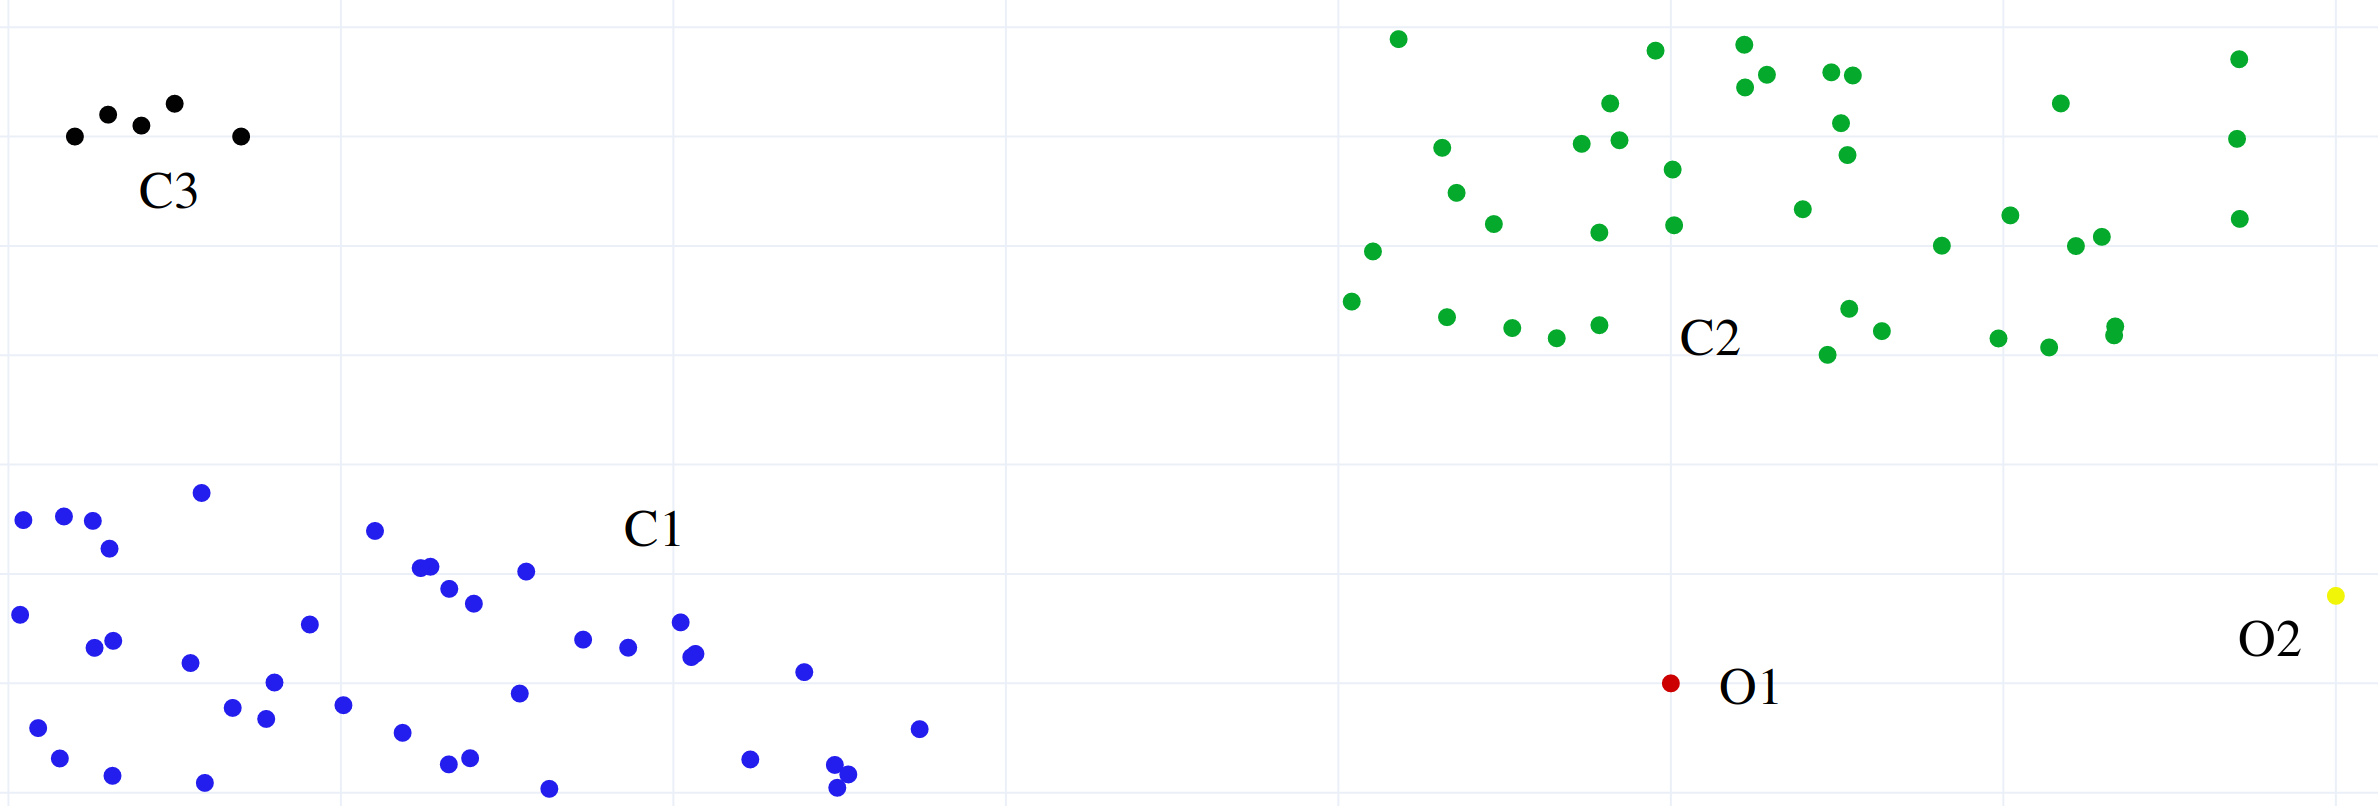
\includegraphics[scale=0.13]{../figures/anomalies.png}
		\caption{Ilustración de tipos de anomalías en un entorno de dos dimensiones}
		\label{fig:anomalias}
	\end{figure}
	
	Podemos encontrar tres tipos diferentes de instancias anómalas~\cite{goldstein2016comparative}:
	
	\begin{itemize}
		\item Anomalía puntual: Es el escenario más frecuente en la detección de anomalías. Las instancias anómalas están completamente aisladas del resto. En la Figura~\ref{fig:anomalias}, O1 y O2 son anomalías puntuales.
		
		\item Anomalía colectiva: La anomalía es una mezcla de varias instancias anómalas. Por ejemplo, la detección de un robo de tarjeta de crédito puede implicar la detección de varios extractos de cuentas bancarias.
		
		\item Anomalía contextual: Una instancia que no es anómala puede serlo dentro de un contexto determinado. Por ejemplo, si medimos la temperatura de un motor en un rango de 50 a 120 grados. Una temperatura de 80 grados parece completamente normal, pero si ese valor se da cuando el motor no tiene carga de trabajo, la temperatura estimada debería ser menor.
	\end{itemize}
	
	Las anomalías están relacionadas con el ruido, pero no hay que confundir ambos conceptos. El ruido tiene el mismo comportamiento descrito en la Figura~\ref{fig:anomalias}, pero, el ruido no tiene interés para el analista de datos mientras que las anomalías sí lo tienen. El ruido se produce por una alteración de los datos, por lo que no refleja la distribución original de los mismos. Además, el ruido perjudica la calidad de los datos y esas observaciones deben ser fijadas o eliminadas~\cite{LibroBigData, GARCIAGIL2019135, garciagilipf}. Las anomalías son información valiosa que debe ser detectada, extraída y analizada.

	La detección de anomalías se utiliza en una gran variedad de dominios, como las redes de sensores~\cite{kraljevski2021machine}, la detección de intrusiones~\cite{kilincer2021machine}, las anomalías industriales~\cite{bayram2021real}, la detección de fraudes con tarjetas de crédito~\cite{forough2021ensemble}, la atención sanitaria~\cite{dwivedi2021novel}, y mucho más~\cite{goldstein2016comparative}. El gran número de dominios que involucran el problema de la detección de anomalías, y el creciente número de sensores en todos los campos está haciendo que la detección de anomalías gane en popularidad.

	En cuanto a la salida de un algoritmo de detección de anomalías, puede ser de dos tipos diferentes~\cite{chandola2009anomaly}:
	
	\begin{itemize}
		\item Etiquetas: El valor de retorno es una etiqueta binaria para cada instancia que indica qué instancias son normales y cuáles son anomalías.
	
		\item Scores: El valor de retorno es una puntuación de anomalía para cada instancia. Dicha puntuación indica la probabilidad de que una instancia sea anómala. También hay que estudiar qué puntuaciones son anómalas.
	\end{itemize}
	
	Como se ha mencionado anteriormente, nos centramos en la detección de anomalías en las series temporales. Una serie temporal es una colección de datos que sigue un orden cronológico. Algunas de sus características son: gran tamaño, alta dimensionalidad y actualización continua. Las series temporales han adquirido una gran importancia, ya que se utilizan en muchos ámbitos, como los datos diarios de temperatura, los datos semanales de ventas, las mediciones de los sensores de los motores u otras máquinas, etc.

	Hay una gran variedad de aplicaciones en el ámbito del problema de la detección de anomalías. La detección de fraudes consiste en encontrar movimientos inusuales en aplicaciones comerciales como bancos, compañías telefónicas, tarjetas de crédito, etc~\cite{forough2021ensemble}. La detección de intrusiones se refiere a la detección de actividades anómalas en una red informática~\cite{kilincer2021machine}. Debido a la gran cantidad de flujo de información, puede producirse un elevado número de falsas alarmas. Esos movimientos inusuales están relacionados con intentos de robo de identidad o de una persona. Además, la detección de anomalías puede aplicarse en el mundo de la industria, detectando algunos daños en las estructuras, errores de instrumentación de los sensores de los motores o comportamientos inesperados en los motores de una cadena de montaje~\cite{bayram2021real}.
	
	Otras aplicaciones de interés son la detección de anomalías en datos de texto, la detección de anomalías en redes de sensores~\cite{kraljevski2021machine} o el procesamiento de imágenes~\cite{pang2021deep}.
	
	\subsection{Evaluación de los problemas de detección de anomalías}
	
	Para analizar el rendimiento de un algoritmo de detección de anomalías, se suelen utilizar cuatro métricas, que se representan en la matriz de confusión que se muestra en la Tabla~\ref{tab:confusion-matrix}. Tanto los verdaderos negativos como los verdaderos positivos son los valores más importantes y considerados, representan que el modelo está acertando en la predicción. El problema surge cuando el número de falsos positivos o falsos negativos es elevado. Hay dos medidas principales calculadas a partir de la matriz de confusión, la sensibilidad~\ref{eq:sensibilidad} que indica la capacidad de etiquetar como positivos los verdaderos positivos, y la especificidad~\ref{eq:especifidad} que indica la capacidad de etiquetar como negativos los verdaderos negativos.
	
	\begin{equation}
		\label{eq:sensibilidad}
		\frac{TP}{TP+FN}
	\end{equation}
	
	\begin{equation}
		\label{eq:especifidad}
		\frac{TN}{TN+FP}
	\end{equation}
		
	Sin embargo, existe un equilibrio entre ambas medidas, ya que el aumento de una de ellas implica la disminución de la otra, por lo que encontrar el mejor ajuste posible es una tarea difícil y dependerá del problema a tratar qué medida tendrá prioridad.
	
	Existe otro equilibrio entre $TPs$ y la tasa de falsos positivos~\ref{eq:equilibrio}.
	
	\begin{equation}
		\label{eq:equilibrio}
		FPR = \frac{FP}{FP+TP}
	\end{equation}
	
	El aumento de $TPs$ suele dar lugar a un mayor $FPR$ porque se da más importancia a las observaciones positivas y, por tanto, aunque se etiqueten correctamente más observaciones positivas, las observaciones negativas también se etiquetarán como positivas. Una característica distintiva de los problemas de detección de anomalías es que el número de observaciones normales es mucho mayor que el número de observaciones anómalas, por lo que intentar ajustar el modelo para centrarse en las observaciones anómalas da lugar a un incremento del número de falsos positivos, generando así alarmas innecesarias. Además, es posible que una observación sea etiquetada como positiva cuando no lo es en función de su contexto (dando lugar a un falso positivo), lo que es común cuando se trata de un problema de series temporales \cite{hundman2018detecting, sridhar2014model}. 
	
	\begin{table}[htb]
		\centering
		\resizebox{\textwidth}{!}{
			\begin{tabular}{cccc}
				\multicolumn{2}{c}{\multirow{2}{*}{}} & \multicolumn{2}{c}{Predicción} \\
				\multicolumn{2}{c}{} & Negativos & Positivos \\ \cline{3-4} 
				\multirow{2}{*}{Valor Real} & \multicolumn{1}{c|}{Negativos} & \multicolumn{1}{c|}{Verdaderos Negativos (TN)} & \multicolumn{1}{c|}{Falsos Positivos (FP)} \\ \cline{3-4} 
				& \multicolumn{1}{c|}{Positivos} & \multicolumn{1}{c|}{Falsos Negativos (FN)} & \multicolumn{1}{c|}{Verdaderos Positivos (TP)} \\ \cline{3-4} 
			\end{tabular}
		}
		\caption{Matriz de confusión}
		\label{tab:confusion-matrix}
	\end{table}
	
	\bibliography{M6_Lopez_Pretel_David}
	\bibliographystyle{plain}
	
\end{document}